\documentclass[10pt]{article}

\usepackage{microtype}
\usepackage{graphicx}
\usepackage{subfigure}
\usepackage{booktabs}
\usepackage{mathtools}

\usepackage{fontawesome}
\usepackage{hyperref}
\usepackage{url}

\usepackage{lipsum}
\usepackage{listings}
\usepackage{graphicx}
\usepackage{color}
\usepackage{amsmath}
\usepackage[]{algorithm2e}

\usepackage{amssymb}
\usepackage[table,xcdraw]{xcolor}

% Attempt to make hyperref and algorithmic work together better:
\newcommand{\theHalgorithm}{\arabic{algorithm}}

\usepackage[accepted]{icml2020}

\usepackage{listings}
\usepackage{xcolor}

\usepackage{makecell}

\definecolor{codegreen}{rgb}{0,0.6,0}
\definecolor{codegray}{rgb}{0.5,0.5,0.5}
\definecolor{codepurple}{rgb}{0.58,0,0.82}
\definecolor{backcolour}{rgb}{0.95,0.95,0.92}

\lstdefinestyle{mystyle}{
    backgroundcolor=\color{backcolour},   
    commentstyle=\color{codegreen},
    keywordstyle=\color{magenta},
    numberstyle=\tiny\color{codegray},
    stringstyle=\color{codepurple},
    basicstyle=\ttfamily\footnotesize,
    breakatwhitespace=false,         
    breaklines=true,                 
    captionpos=b,                    
    keepspaces=true,                 
    numbers=left,                    
    numbersep=5pt,                  
    showspaces=false,                
    showstringspaces=false,
    showtabs=false,                  
    tabsize=2
}

\lstset{style=mystyle}

\begin{document}

\twocolumn[
\icmltitle{Deep Clustering of Event Sequences}

\icmlsetsymbol{equal}{*}

\begin{icmlauthorlist}
\icmlauthor{Vlad Zhuzhel}{sk}
\icmlauthor{Evgeny Lagutin}{sk}
\icmlauthor{Anna Rudenko}{sk}
\icmlauthor{Liliya Mironova}{sk}
% \icmlauthor{Example}{equal,other}
\end{icmlauthorlist}

\icmlaffiliation{sk}{Skolkovo Institute of Science and Technology, Moscow, Russia}
% \icmlaffiliation{other}{Other affiliation}

\icmlcorrespondingauthor{Rodrigo Rivera-Castro}{rodrigo.riveracastro@skoltech.ru}

\icmlkeywords{Final Project, Model of Sequence Data, Skoltech}

\vskip 0.3in
]
\printAffiliationsAndNotice{}  % leave blank if no need to mention equal contribution
% \printAffiliationsAndNotice{\icmlEqualContribution} % otherwise use the standard text.
\begin{abstract}
Clustering temporal point processes is a challenging task due to the random nature of the point processes. There are a lot of methods for supervised and unsupervised classification of classical (synchronous) time-series. For asynchronous time-series or temporal point processes, there are almost no methods that exist right now. Dirichlet Hawkes Mixture Model allows to do unsupervised classification, however, this method is parametric. In this work, the novel Cohortney method has been taken and some different neural approaches have been used for clustering. That allowed to do non-parametric learning and achieve good results on both synthetic and real-data datasets. \footnote{\href{https://github.com/rodrigorivera/mds20\_cohortney}{github.com/rodrigorivera/mds20\_cohortney}}
\end{abstract}

\section{Introduction}\label{sec:intro}
In the world, there are a variety of processes that can be considered temporal point processes, e.g. actions on tweets, watching one of the channels with TV, activity on websites, accidents, the electronic health records in a hospital and many others. Indeed, all these processes can correspond to several clusters, for example, the website users can be loyal or non-loyal. In many cases, we don't have labels and need to perform learning in an unsupervised manner.

There are many well-established methods for synchronous data clustering with discrete time-lags of observations \cite{surv_ts_clus}. However, there are few methods for clustering temporal point processes. The reason is that this data is in the continuous time domain, and it is hard to find the representation of this data. Also, the random nature of these processes makes it hard to learn clusters on this data. 

The only existing solution in our notion that solves this problem is a Dirichlet Mixture Model of Hawkes Processes\cite{123dirichlet}. The main idea of this method is to consider the Hawkes process parameters to be random variables and then learn the parameters in an expectation-maximization manner. The main drawback of this method, in our opinion, is that it has a parametric assumption and that these processes are Hawkes processes. 

In this work, we propose non-parametric methods for temporal point processes clustering. To do so, we propose to use Cohortney partitions and then use different deep learning clustering techniques to obtain these clusters. It has been shown that this method allows us to obtain good clusters even if we consider small partitions and, in some cases, it can outperform DMHP algorithm.

The main contributions of this report are as
follows:

\begin{itemize}
    \setlength{\parskip}{0pt}
    \item We successfully adopted a state-of-the-art unsupervised method proposed for image classification to event sequences classification task. 
    \item We implemented different architectures for event sequences classification.
    \item We compared the performance of different architectures.
\end{itemize}

\section{Preliminaries}\label{sec:prelim}

Asynchronous sequential data is a kind of information that one may consider to analyze. The conventional example is an IPTV system. A common model covering most of the sequential data examples is called the event sequences model. Each sequence consists of events of different types in continuous-time. Clustering of these event sequences may be beneficial to the data owner: e.g. TV company is interested in clustering IPTV users to suggest ads to them according to their preferences.  

% We have a post $p=(a_1, a_2\dots a_k)$ where $a_k$ is comment, which appeared in post.  We should predict a moment when thr next comment appears. So we should perform clustering and calculate the optimal time $\tau^{\ast}$ (time when comment appears) for each cluster


% The posts in social networks may be considered as temporal point processes. 

% These are the processes of event sequences $\{(t_i, c_i)\}_{i=1}^M$ with timestamps $t_i$ and event types $c_i \in \mathcal{C} = \{1,\dots,C\}$.

% These are the processes of event sequences $\{(t_i, c_i)\}_{i=1}^M$ with timestamps $c_i$ and event types $c_i \in \mathcal{C} = \{1,\dots,C\}$, where $c_k$

A temporal point process is a random process whose realization consists of an event sequence $\left\{\left(t_{i}, c_{i}\right)\right\}_{i=1}^{M}$ with timestamps $t_{i} \in[0, T]$ and event types $c_{i} \in \mathcal{C}=\{1, \ldots, C\} .$ It can be equivalently represented as $C$ counting processes $\left\{N_{c}(t)\right\}_{c=1}^{C},$ where $N_{c}(t)$ is the number of type-$c$ events occurring at or before time $t$. A way to characterize point processes is via the intensity function $\lambda_{c}(t)=\mathbb{E}\left[d N_{c}(t) \mid \mathcal{H}_{t}^{\mathcal{C}}\right] / d t,$ where $\dot{\mathcal{H}}_{t}^{\mathcal{C}}=\left\{\left(t_{i}, c_{i}\right) \mid t_{i}<t, c_{i} \in \mathcal{C}\right\}$ collects historical events of all types before time $t$.

One of the simplest types of point processes is Poisson process. In this case every event type has intensity $\lambda_c$ and the probability of the event to occur is $P(t_i^c \in [t,t+dt)) = \lambda_ dt$. Also one can consider homogeneous Poisson process, when $\lambda \neq \mathrm{const}$ and $\lambda(t) \geq 0$.

However, in this case, the appearance of the new event doesn't depend on history. One of the generalizations is the Hawkes process.

In Hawkes process we assume that the history of the events can influence the intensity function:

\begin{equation}
    \lambda_c(t) = \mu_c + \sum_{t_i<t} \phi_{cc_i}(t-t_i), ~ \mu_c \geq 0, ~ \phi_{cc'}(s) \geq 0
\end{equation}

$\mu_c$ is a base intensity, $\phi_{cc'}(s)$ are so called impact functions or kernels. 

Let's assume that one has $K$ type of Hawkes processes and a set of event sequences $\mathbf{S} = \{\mathbf{s}_n\}_{n=1}^N$, $\mathbf{s}_n = \{(t_i,c_i)\}_{i=1}^{M_n}$, $c_i \in \mathcal{C} = \{1,\dots,C\}$ and $t_i \in [0,T_n]$. Each event sequence corresponds to one of $K$ types of Hawkes processes with its intensity function.

One needs to perform clustering of the given set of event sequences.

\section{Related work}\label{sec:related}

As has been said there are few methods for the unsupervised classification of temporal point processes. In this work, we have used DMHP as a baseline and compared the performance with the performance of this method.

\subsection{Dirichlet Mixture Model of Hawkes Processes}\label{sec:dmhp}
There are not many works doing clustering of event sequences and it seems to be no fully-fledged comparison of existing approaches in this direction. Therefore it is not very clear if there is a real SOTA approach. But still, as our main baseline, we take the method from \cite{123dirichlet}. The authors represent event sequences as Hawkes Processes' realizations. The model looks as follows:

\begin{equation}
\lambda_{c_i}^k(t_i) = \mu_{c_i}^k + \sum_{t_j<t, d}a_{c_i,c_j,d}^kg_d(t-t_j)
\end{equation}

, where $g_d$ - basis functions that are Gaussians in the original paper, $\mu_{c}^k,~a_{c,c',d}^k$ - parameters of the model, $k\in 1..K$ - cluster indexes.

In the proposed mixture model, the probability of the appearance of an event sequence $s$ is

\begin{align}
p(\boldsymbol{s} ; \boldsymbol{\Theta})&=\sum_{k} \pi^{k} \mathrm{HP}\left(\boldsymbol{s} \mid \boldsymbol{\mu}^{k}, \boldsymbol{A}^{k}\right), \\ \mathrm{HP}\left(\boldsymbol{s} \mid \boldsymbol{\mu}^{k}, \boldsymbol{A}^{k}\right)&=\prod_{i} \lambda_{c_{i}}^{k}\left(t_{i}\right) \exp \left(-\sum_{c} \int_{0}^{T} \lambda_{c}^{k}(s) d s\right)
\end{align}

Here $\text{HP}$ - PDF of Hawkes Process, $\pi^{k}$’s are the probabilities of clusters.
They propose learning parameters of each cluster with the nested EM algorithm. For that purpose, they introduce $\pi^k$ - probabilities of each cluster. Therefore the likelihood of each sequence is a mixture of Hawkes processes. An important assumption the authors make in their paper is that $\mathbf{\mu}^k, \mathbf{A}^k$ are random variables and $\mathbf{\pi}$ is a random vector that obeys Dirichlet distribution. Their motivation for inducing priors for $\mu$ and $A$ is that they have to preserve some physically-meaningful constraints. It is not absolutely clear why do authors need clusters to have Dirichlet prior or any prior at all. As a consequence, they use variational Bayesian inference to learn both the parameters of each model and their priors. Not going deep into details the joint distribution is factorized as

\begin{equation}
p(S, Z, \mathbf{\pi}, \mathbf{\mu}, \mathbf{A}) = p(S|Z, \mathbf{\mu}, \mathbf{A})p(Z|\mathbf{\pi})p(\mathbf{\pi})p(\mathbf{\mu})p(\mathbf{A})
\end{equation}

\begin{align}
p(S|Z, \mathbf{\mu}, \mathbf{A}) &= \prod_{n,k}\text{HP}(s_n|\mathbf{A}^k \mathbf{\mu}^k)^{z_{nk}} 
\\ p(Z|\mathbf{\pi}) &=\prod_{n,k}(\pi^{k})^{z_{nk}}
\end{align}

Here $S$ are $N$ available event sequences, $Z \in \{0, 1\}^{N\times K}$ - matrix of labels. 

To learn the above model authors propose using EM algorithm applied to a variational distribution $q(Z,\mu, A, \pi)=q(Z)q(\pi, \mu, A)=q(Z)q(\pi)\prod_k \q(\mu^k)q(A^k)$ . At each E-step of the loop, they evaluate the expected value of $\log q^*(Z)$ and at M-step they evaluate the parameters $\mu, A$ maximizing the term $q(\pi, \mu, A)$ and update their priors, assuming $\mu, A$ to be equal to their expectation. It worth saying that inside the M-step it is needed to conduct an optimization procedure to obtain optimal $\mu$ and $A$ and therefore authors provide an explicit iterative procedure that is inner EM loop at each M-step of the outer loop. Besides the main framework for clustering, the authors propose a way to update the number of clusters during the algorithm running. Moreover, they prove a theorem that under mild assumptions their mixture model is locally identifiable, meaning that for each set of parameters and cluster probabilities there is an open neighborhood containing no other set, such that likelihood given those two sets match for any possible sequence. 

The authors provide a comparison of their method to several other approaches that may be described in a similar way: they choose a way to learn representations of the event sequences and apply the Dirichlet Process Gaussian Mixture Model \cite{krueger2018dirichlet} to perform clustering. According to the paper \cite{123dirichlet}, the solution proposed by the authors allows to get higher consistency of clustering on the unlabeled real-world data (IPTV dataset). 



% One may consider the following questions arising: Do we really need fully Bayesian model as proposed in the paper or it is possible to get comparable results without making a plenty assumptions on parameters and clusters distributions? If yes, wouldn't it be beneficial to use neural intensity function instead of combination of Gaussians and perform the EM algorithm for clustering but using for example gradient methods at the M-step? As a possible next step we consider to evaluate the combination of  Neural Hawkes and EM algorithm without Bayesian assumptions (for simplicity) as an alternative baseline.

\subsubsection{Implementation}
The authors have a repository containing a library of methods for learning point processes implemented using Matlab. Unfortunately, there are no Matlab experts among our team. We provide a PyTorch implementation of DMMHP in our repository. As reproducing the approach completely is not our main goal our implementation has several specifications. First, we don't reproduce the tuning of basic function parameters as described in the original paper. Second, we encountered a problem when computing negative log-likelihood because as we understand there is no straightforward way to compute it for Hawkes mixture without computing likelihood directly. But when doing it we need to compute the product of many (length of sequence) items and therefore we get an overflow error. Thus in our implementation, we skip all the steps using the computation of negative log-likelihood. 

\subsection{Deep Learning methods for Unsupervised Learning}
Cohortney algorithm allows us to obtain partitions and then find the similarity between different time-series, comparing their partitions. However, this method doesn't take into account that point-processes with different partitions can be from the same cluster and also that there can be some hidden similarities that in general can be described with intensity function.

To partly overcome these issues we propose to use different deep learning techniques on top of Cohortney partitions and assume that Neural Networks can catch these hidden similarities. To do so we consider autoencoders that have been proven to be good in representation learning and also adjust two methods \cite{guo2017deep} and \cite{asano2020self} that has shown great performance on image clustering.

More about these methods will be said in Algorithms and Models as soon they have been used for learning.
% In our github repository we provide not finished yet PyTorch implementation of DMMHP. We are on the way to reproduce the results on the IPTV dataset presented in the original paper. One of the problems we encountered during reproducing methods from \cite{123dirichlet} is related to that they make a range of assumptions on parameters and cluster distributions and provide the EM framework based on the corresponding calculations. Therefore it is quite possible to make a mistake while transferring their ideas from the paper to the code as there is no easy way to check the correctness of the intermediate computations.

\section{Algorithms and Models}\label{sec:algos}

%\subsection{Cohortney}
%\subsubsection{Description of the method}

%\subsubsection{Implementation}


\subsection{Cohortney}\label{sec:cohortney}
\paragraph{}
In this section, we have implemented two algorithms presented in Cohortney manuscript. In order to make the text below more clear let's introduce some parameters, we are going to use. The first parameter is an event sequence $p$ (in this work we consider one post to be an event):
\begin{equation}
    p = (a_1, a_2, \dots, a_n),
\end{equation}
where $a_i$ - is a time when the comment under the post appears. We have a bunch of such posts, our source data:
\begin{equation}
    P = (p_1, p_2, \dots, p_n).
\end{equation}
We need to clusterize all these events from $P$ into different clusters. Let there be the parameter t, which we call the present moment. This parameter is fixed, and no comment is considered to be posted after $t$: $a_n \leq t$.  We have an an arbitrary time interval $(t_1 , t_2)$ and $n$ events (comments) may happen in this interval. Thus we can introduce the weight function:
\begin{equation}
\label{eqn:fws}
    fws(p, t_1, t_2) =  \min ([\log_2 (n+1)], 9).
\end{equation}
Now let's define a weight function for the entire time sequence. Let's call the partition $\Delta T^*$ on the half interval $(0, t]$ the function with the following form:
\begin{equation}
    \Delta T^* = \{t_0, t_1, \dots, t_m\}, 0=t_0 \leq t_1 \leq \dots \leq t_m =t
\end{equation}

The distance between the adjacent elements is $\Delta t_n$ which can be computed as:
\begin{equation}
    \Delta t_n = \frac{T^*}{2^n}
\end{equation}
Hence the weight function for the entire time sequence can be computed the following way:
\begin{equation}
\label{eqn:fws_interval}
    fw(p, t, \Delta T^*) = \{fws(p, t_0, t_1), \dots, fws(p, t_{m-1}, t_m)\}
\end{equation}


After this brief introduction let's introduce two algorithms: Cohort1, and Cohort2. Depending on time partition $\Delta T_J$ and current moment $T_j$ cohort1 computes triplets for each event from $P$. Then, based on triplets, we put an event to a specific cluster, one event may be in several classes. We arrange this using \texttt{dict} structure in Python.

Cohort2 computes a bunch of triplets for a new incoming event, then it compares its triplet to the already obtained triplets in order to find the closest cluster to this new event.




\subsubsubsection{COHORT 1}
\begin{algorithm}
 \KwData{$P$}
 \KwResult{Set of clusters}
 initialization\;
 \For{$T_j$ in grid}{
  Compute the partition $\Delta T_j^n$\;
  \For{$p_k$ in $P$}{
  Compute the triplet $(T_j, \Delta T_j^n, fw(p_k,\Delta T_j^n)$\;
  Group the $p_k$ by it's triplet\;
  \If{cluster size < N}{
   Dicard this cluster\;
   
   }
  }
 }

\caption{COHORT1}
\end{algorithm}
 
In this algorithm, we get the set of clusters from the bunch of events.

\subsubsubsection{COHORT2}
\begin{algorithm}[H]
 \KwData{$p_i$, $t$}
 \KwResult{Nearest cluster }
 Find the nearest node $T_t$ to $t$ that does not exceed $t$ \;
 \For{$i$ in $n$}{
  Compute the triplet $(T_j, \Delta T_j^n, fw(p_k,\Delta T_j^n)$\;
  }
  \For{$triplet$ in $clusters$}{
  n = 0\;
  Find the closest cluster\;
  Group the $p_k$ by it's triplet\;
  n = n+1\;
  
  \If{no cluster}{
   Take n-1 as a closest cluster\;
   
   
  }
 }
\caption{COHORT2}
\end{algorithm}
In this algorithm, we find the closest cluster from the already existed clusters for a new event sequence.

\paragraph{}
As you can see both these algorithms are vague and leave room for speculations, ideas. This Cohort part will be modified in the next iterations of our projects. For the first iteration of our project, we have implemented a verbatim model in order to understand how these algorithms work. 

So the first implementation is a cyclic implementation with brute-force. We used $ticks$ library in order to implement a synthetic toy dataset to tune the baseline. From our synthetic dataset, we calculated a triplet for every event. And thus, on every iteration, we get a bunch of $n$ triplets for every event $p$. In order not to produce any clustering algorithm after the cohort1 we decided to use a dictionary structure in python, which allowed us to use a specific triplet as a key and set of the events with this triplet as a value of this. Thus we automatically receive the clusters. After the Cohort1 finishes, its work we discarded all the clusters, where we have less than $N$ events.

For the Cohort2 we should generate a new event, which we generate with \texttt{tick} library. We randomly choose the value of $t$. Then we compute triplets for each possible partition. Then, by brute-force, we find if we compare our clusters to the clusters we obtained from Cohort1. That's how we find the closest or the coinciding cluster for our new event. This spot is now implemented by word, but I suppose we may increase the speed of this cycle by applying any sorting algorithm for strings. The task of finding the nearest cluster in these terms may be reduced to string sorting. This idea, besides the deep implementation of this part, will be checked in the next iteration of our project.

\subsection{Clustering with Convolutional Autoencoders}\label{sec:CAE}
One of the ideas, how to cluster the sequences using COHORTNEY was deep clustering with convolutional autoencoders. This  well-known and widely used method   was offered in \cite{guo2017deep}. In the original paper \cite{guo2017deep} the clustering process was performed on 3D tensors (pictures) and 2D convolutions were used.
A conventional autoencoder is generally composed of two layers, corresponding to encoder $f_w(·)$ and decoder $g_U(·)$ respectively. It aims to find a code for each input sample by minimizing the mean squared errors (MSE) between its input and output over all samples, i.e.
\begin{equation}
    \label{eqn: mse}
    \min_{W, U} \frac{1}{n} \sum_{1}^{n} \|g_u(f_W(x_i)) - x_i\|_{2}^{2}
\end{equation}

For fully connected autoencoder we obtain
\begin{equation}
\label{eqn: }
    \begin{array}{cc}
         &  f_W(x) = h\\
         & g_U(h) = \hat{x}
    \end{array}
\end{equation}
Where $h$ is latent feature representaion, $\hat{x}$ is model prediction. 
Convolutional Autoencoders (CAE) were trained in end-to-end manner for learning features in unlabeled images.
\begin{figure}[h!]
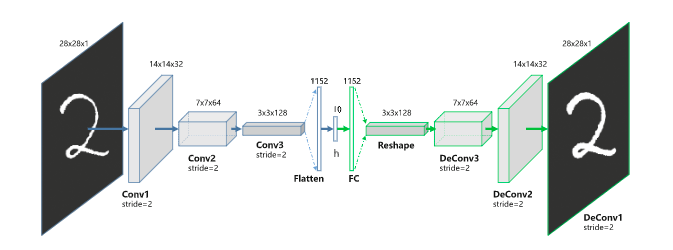
\includegraphics[width=8cm]{Final_Project_Guidelines_Source/figs/CAE.png}
\caption{ Convolutional AutoEncoders (CAE) for MNIST.}
\label{fig:CAE}
\centering
\end{figure} 

Then, a clustering oriented loss is directly built on embedded features to jointly perform feature refinement and cluster assignment.
\paragraph{}
In our case, we have 1D tensors of the weight function \ref{eqn:fws_interval}. We decided to use 1D Convolutional autoencoders in order to get latent features and cluster them with the KMeans algorithm. The basic idea was to train a 1D convolutional autoencoder with MSE \ref{eqn: mse} loss and then to get latent feature representation from the encoder. As we have multiclass sequences in our IPTV and simulated Hawkes datasets, the initial amount of classes was considered as the input features. Then, after getting the latent features from the encoder, we pass the reshaped latent data to the Kmeans algorithm.

\subsubsection{Implementation}

We have implemented a 1D convolutional autoencoder using \texttt{Pytorch Lightning} framework. This framework is a wrapper over the \texttt{Pytorch} in order to speed up this library. The structure of the convolutional autoencoder is straightforward: it consists of 5 1D convolutions with Batch Normalization in between. We used the default setting for torch convolutional layer: stride equals to $1$ and padding equals $0$. Kernel size was set to $3$. In order to cluster the encoder output we used standard \texttt{sklearn} library with \texttt{kmeans} algorithm.


\subsection{Deep Clustering}\label{sec:deep_cluster}
Given partitions obtained from Cohortney for a particular $n$ we may proceed with clustering algorithms suitable for sequences of features of the same length. Therefore we try to combine Cohortney with a couple of deep learning approaches for object clustering. The first one we describe here is a method for image clustering proposed in \cite{DBLP:journals/corr/abs-1807-05520} that is called Deep Clustering. 

\begin{figure}[h!]
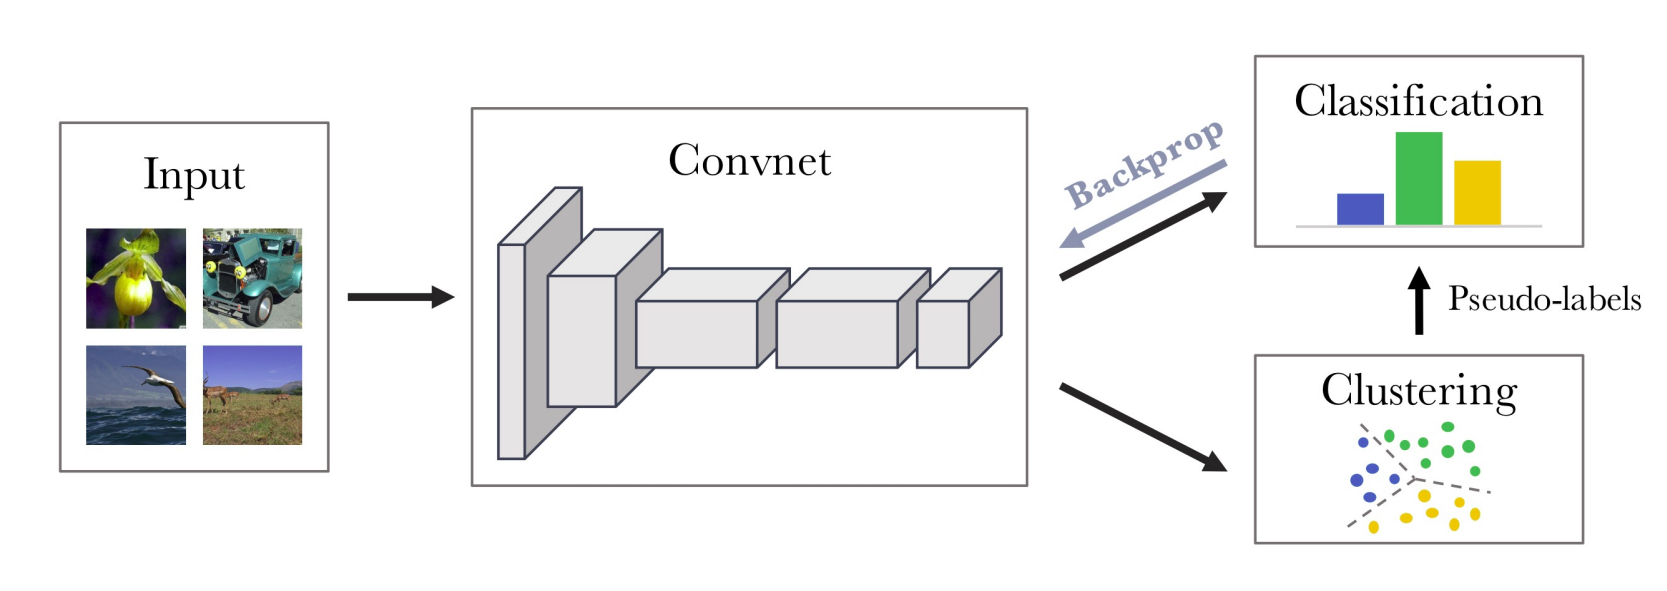
\includegraphics[width=8cm]{Final_Project_Guidelines_Source/figs/deep_cluster.png}
\caption{ Illustration of the Deep Clustering}
\label{fig:deep_cluster}
\centering
\end{figure} 

The basic idea of the approach is described in the Figure \ref{fig:deep_cluster}. We denote by $f_{\theta}$ the convnet mapping, where $\theta$ is the set of corresponding parameters. We refer $f_{\theta}(x)$ to the vector obtained by applying this mapping to a sequence. Given a training set $X=\left\{x_{1}, x_{2}, \ldots, x_{N}\right\}$ of $N$ sequences (in Cohortny partition representation $f_w$), we want to find a parameter $\theta^{*}$ such that the mapping $f_{\theta^{*}}$ produces good general-purpose features.

These parameters are traditionally learned with supervision, i.e. each sequence $x_{n}$ is associated with a label $y_{n}$ in $\{0,1\}^{k} .$ This label represents the image's membership to one of $k$ possible predefined classes. A parametrized classifier $g_{W}$ predicts the correct labels on top of the features $f_{\theta}\left(x_{n}\right) .$ The parameters $W$ of the classifier and the parameter $\theta$ of the mapping are then jointly learned by
Deep Clustering for Unsupervised Learning of Visual Features
optimizing the following problem:

\begin{equation}
\min _{\theta, W} \frac{1}{N} \sum_{n=1}^{N} \ell\left(g_{W}\left(f_{\theta}\left(x_{n}\right)\right), y_{n}\right)
\end{equation}

where $\ell$ is the multinomial logistic loss, also known as the negative log-softmax function. This cost function is minimized using mini-batch stochastic gradient descent and backpropagation to compute the gradient.

More specifically the training consists of the following steps. On each epoch of the training phase, deep features of sequences are computed with convnet. These features are used to cluster sequences using the KMeans algorithm. The top fully-connected classifier is then initialized and put onto the top of the model. The obtained pseudolabels are then used for supervised-manner training of the model.  


\subsubsection{Implementation}
We adopt the original implementation of the Deep Clustering. We use \texttt{sklearn} implementation of KMeans algorithm with \texttt{kmeans++} initialization. We standardize features with \textt{sklearn} realization of \texttt{StandardScaler} before clustering. One of the drawbacks of this approach we observed is that there is no guarantee of convergence of assigned clusters and in fact, the quality of clustering may change dramatically during training. As a consequence of this feature is that the variation of the clustering quality may be huge. Besides we observe that the algorithm is highly sensitive to change of hyperparameters. 

\subsection{Optimal Transport}\label{sec:ot}
In this work, we adopted a state-of-the-art approach for image unsupervised classification proposed in \cite{asano2020self}. The idea of the approach is to do representation learning and clustering at the same time. It has shown to be effective for images and in this work we are using the same technique for event sequences clustering.

So let's consider the problem of unsupervised classification for some instances $I$. Let's consider the NN combing the representation NN $x = \Phi(I)$ and a classification head $h$. So $x$ will be a feature vector. Each data point $I_1,\dots, I_N$ has corresponding label $y\in\{1,\dots,K\}$. The model should map from the data points space to the scores of each class, which can be considered as probability after applying a softmax operator.

\begin{equation}
    p(y = \cdot|\mathbf{x}_i) = \mathrm{softmax}(h  \circ \Phi(\mathbf{x}_i))
\end{equation}

In this case the cross-entropy loss will be:

\begin{equation}
    E(p|y_1,\dots,y_n) = - \frac{1}{N}\sum_{i=1}^N \log p(y_i|\mathbf{x}_i)
\end{equation}

For semi-supervised classification one can consider optimizing loss both with respect to the model and to the labels. However, in the case of unsupervised learning, this will lead to a degenerate solution. So it was proposed to introduce the posterior distribution $q(y|\mathbf{x}_i)$ and to additionally constraint the clustering with equipartition. Then the problem can be written as follows:
\begin{equation}
    \begin{split}
       E(p,q) = -\frac{1}{N}\sum_{i=1}^N&\sum_{y = 1}^K q(y|\mathbf{x}_i)\log p(y|\mathbf{x}_i)\\
       \min_{p,q} E(p&,q)\text{ subject to }\\ \forall y: q(y|\mathbf{x}_i) \in \{0,1&\} \text{ and } \sum_{i=1}^N q(y|\mathbf{x}_i)=\frac{N}{K}
    \end{split}
\end{equation}

Let's denote $P_{yi} = p(y|\mathbf{x}_i)\frac{1}{N}$ and $Q_{yi} = q(y|\mathbf{x}_i)\frac{1}{N}$. Let's relax matrix $Q$ to be an element of the transportation polytope:
\begin{equation}
U(r,c) = \{Q\in \mathbb{R}_{+}^{K\times N}|Q\mathbf{1} = r, Q^{\top} \mathbf{1} = c\}
\end{equation}

Vector $\mathbf{1}$ denotes all ones of appropriate dimensions.

\begin{equation}
    r = \frac{1}{K}\mathbf{1}, \text{ }c = \frac{1}{N}\mathbf{1}
\end{equation}

In this case the objective function can be rewritten as:

\begin{equation}
    E(q,p) + \log N = \langle Q, -\log P\rangle
\end{equation}

So the optimization is equivalent to solving the minimization problem:

\begin{equation}
    \min_{Q\in U(r,c)} \langle Q, - \log P \rangle
\end{equation}

This is a transport problem and this problem can be solved in polynomial time, however for big datasets, it can be inefficient, that's why it was proposed to use a fast Sinkhnorn-Knopp algorithm. In this case, the objective function also has a regularization term:
\begin{equation}
    \min_{Q\in U(r,c)} \langle Q,-\log P \rangle + \frac{1}{\lambda} \mathrm{KL}(Q||rc^{\top})
\end{equation}

Minimizer of the equation is $Q =\mathrm{diag}(\alpha)P^{\lambda}\mathrm{diag}(\beta)$. Here the exponentiation is elementwise and vectors $\alpha$ and $\beta$ a chosen so that the resulting matrix was a probability matrix. Choosing $\lambda$ is a tradeoff between the convergence speed and the closeness to the original problem.

So the optimization consists of two steps. For a given label assignment optimizing the model with respect to the parameters. And then given the probabilities $P$ update iteratively  $\alpha$ and $\beta$ with the following formulas:

\begin{equation}
    \forall y: \alpha_y \leftarrow [P^{\lambda}\beta]_y^{-1} \text{, } \forall i: \beta_i \leftarrow [\alpha^{\top}P^{\lambda}]_i^{-1}
\end{equation}

\subsubsection{Implementation}

The code from \cite{asano2020self} has been used as a reference. To train the model the following approach has been used. Given the maximal time $T_h$ the following partitions has been used:
\begin{equation}
    (T_j, \Delata T_j(T_j/2^k), fws),~ T_j = T_h/2^n
\end{equation}

Here $k, ~ n$ take values from $0$ to some hyper-parameters $K, ~N$. Then we train convolutional filters followed by linear layer and predicting linear layer on top of these partitions.

\section{Experiments and Results}\label{sec:exp_res}
\subsection{Data}
For our experiments, we used the real-world Internet Protocol Television (IPTV)  dataset of $300$ event sequences - one per user - and a range of synthetic datasets collected using the library for simulating Hawkes processes \texttt{tick}.
You may download the IPTV dataset via the following link: \href{https://github.com/rodrigorivera/mds20_cohortney/raw/main/data/IPTV_Data.zip}{IPTV\_Data.zip}

Following \cite{123dirichlet} we generated $5$-dimensional realizations of Hawkes processes for $3$, $4$, $5$ clusters ($3$ datasets). We generated $400$ realizations per each cluster. You may download all synthetic  datasets via the following link: \href{https://github.com/rodrigorivera/mds20_cohortney/raw/main/data/simulated_Hawkes.zip}{simulated\_Hawkes.zip}

Here we place the snippet of \texttt{Python} code that we use for data generation:

\lstinputlisting[language=Python, caption=Snippet of synthetic data generation]{Final_Project_Guidelines_Source/code/simulate_hawkes.m}


\subsection{Evaluation}
For our experiments, we adopt the evaluation proposed in \cite{123dirichlet}. As for the IPTV dataset, there are no real labels it is not possible to measure the correctness of clustering. Therefore authors propose to measure the clustering consistency via a cross-validation method. The principle is simple: because random sampling does not change the clustering structure of data, a clustering method with high consistency should preserve the pairwise relationships of samples in different trials. We test each clustering method with $J(=10)$ trials. In the $j$-th trial, data is randomly divided into two folds. After learning the corresponding model from the training fold, we apply the method to the testing fold. We enumerate all pairs of sequences within the same cluster in the $j$ -th trial and count the pairs preserved in all other trials. The clustering consistency is the minimum proportion of preserved pairs over all trials:
$$
\text { Consistency }=\min _{j \in\{1, \ldots, J\}} \sum_{j^{\prime} \neq j} \sum_{\left(n, n^{\prime}\right) \in \mathcal{M},} \frac{1\left\{k_{n}^{j^{\prime}}=k_{n^{\prime}}^{j^{\prime}}\right\}}{(J-1)\left|\mathcal{M}_{j}\right|},
$$
where $\mathcal{M}_{j}=\left\{\left(n, n^{\prime}\right) \mid k_{n}^{j}=k_{n^{\prime}}^{j}\right\}$ is the set of sequence pairs within same cluster in the $j$ -th trial, and $k_{n}^{j}$ is the index of cluster of the $n$ -th sequence in the $j$ -th trial.

For the synthetic data with clustering labels, we use clustering purity to evaluate various methods:
$$
\text { Purity }=\frac{1}{N} \sum_{k=1}^{K} \max _{j \in\left\{1, \ldots, K^{\prime}\right\}}\left|\mathcal{W}_{k} \cap \mathcal{C}_{j}\right|
$$
where $\mathcal{W}_{k}$ is the learned index set of sequences belonging to the $k$ -th cluster, $\mathcal{C}_{j}$ is the real index set of sequence belonging to the $j$ -th class, and $N$ is the total number of sequences.

\subsection{Implementation details}
% \subsection{Datasets description}
% IPTV dataset
In all our experiments with DMHP we set the number of outer iterations equal to $10$. The number of inner iterations grows from $2$ to $8$ for the first $7$ iterations and stays $8$ for the last $3$ iterations. We took $5$ Gaussian basis functions with different scales. The replication of experiments with DMHP can be found in our github. 

For Deep Clustering we use a simple convolutional neural network with batch normalizations. For the main part of the model we use Adam optimizer and for the top layer, we use SGD optimizer with a momentum equal $0.9$. We train the model for $30$ epochs with  learning rate=1e-4, weight decay=1e-4. We apply Deep Clustering over features obtained from Cohortney partition with $n=8$. All our experiments were run on the CPU.

For CAE Clustering we use a straightforward convolutional autoencoder with 5 convolutions and batch normalizations between the convolutions.  The kernel size was set to $3$, stride and padding were default. As a training criterion Mean Squared Error (\ref{eqn: mse}) was chosen. We took Adam optimizer with standard parameters. We trained Convolutional Autoencoder with \textt{Pytorch Lightning} framework on 50 epochs. Batch size equals to 100. We applied CAE Clustering over features obtained from Cohortney partition with $n=8$. The number of out channels from the encoder (the size of latent features space) is 12 for all the datasets. CAE was trained on GPU.


\subsection{Results}


To evaluate methods on the IPTV dataset we ran them for $10$ trials to collect assigned labels and compute Consistency. The result is presented in Table \ref{table:1}.

\begin{table}[h!]
\caption{Clustering Consistency on Real-world Data}
\begin{tabular}{c|ccc}
\hline
method    & \textbf{DMHP}   & \makecell{\textbf{Deep} \\\textbf{Clustering}}   & \makecell{\textbf{CAE} \\\textbf{Clustering}}  \\ \hline
IPTV data & 0.3660 & 0.4234 &\textbf{ 0.4241}
\end{tabular}
\label{table:1}
\end{table}

We computed the mean and the standard deviation of Purity over $5$ runs. The result is presented in Table \ref{table:2}. We denote $K$ as a number of clusters and $C$ as a number of classes. 

\begin{table*}
\centering
\caption{Clustering Purity on Synthetic Data}
\begin{tabular}{c|cccc}
\hline
method    & \textbf{DMHP}   & \makecell{\textbf{Deep} \\\textbf{Clustering}}   & \makecell{\textbf{CAE} \\\textbf{Clustering}} & \makecell{\textbf{Optimal Transport} \\\textbf{Clustering}} \\ \hline
K=5, C=5 &  \textbf{.6108}\pm.0495 & .4384\pm.0985  &
.5306\pm.0447 &
.4537\pm.0513\\
K=4, C=5 &  \textbf{.7505}\pm.0212 & .5613\pm.0158    &
.7113\pm.0474 &
.5372\pm0.0295\\
K=3, C=5 &  \textbf{.8723}\pm.0298 & .6945\pm.1023 &
.797\pm.0581 &
.6731\pm0.8203\\

\end{tabular}
\label{table:2}
\end{table*}


We mark results bold when they are \textit{better} than ones of alternative methods.

For CAE clustering we have a parameter we can control - the number of encoder out channels or the size of latent feature space. In order to investigate if the size of latent features space impacts clustering quality, we hold several experiments and average the results. All the experiments were held on the dataset which showed the worst performance on CAE clustering - Synthetic dataset $K=5$, $N=5$.  
\begin{figure}[h]
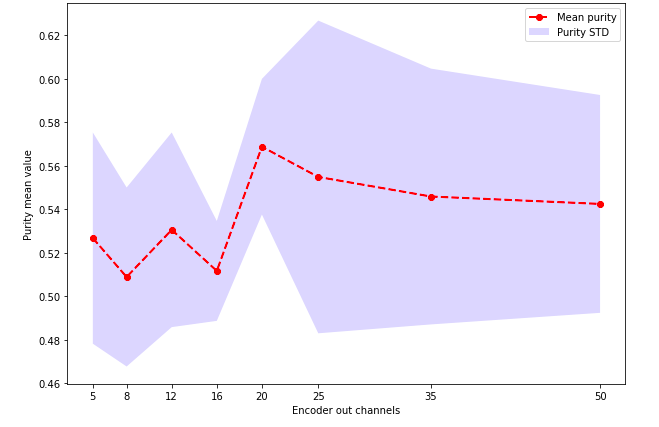
\includegraphics[width=8cm]{Final_Project_Guidelines_Source/figs/outs_more.png}
\caption{ The dependency of purity from the size of latent feature space}
\label{fig:CAEpurity}
\centering
\end{figure} 

We held 5 launches for different sizes of latent feature spaces. For multiclass simulated Hawkes dataset $K=5$, $C=5$ with five clusters the number of encoder out channels were $[5, 8, 12, 16, 20, 25,35, 50]$. As you can on the \ref{fig:CAEpurity} the average purity is set about $0.536$ and does not chanfe significantly. Thus we can conclude that the size of latent features space impacts lightly on the clustering quality.


% \subsection{COHORTNEY}

% \subsection{Deep Clustering}

% \subsection{Optimal Transport}

\section{Conclusion}\label{sec:conclusion}

We could not beat a baseline model for synthetic Data, but we could come up with better results on real world IPTV dataset. All the proposed models came up with adequate results, and these models are non-parametrical, what is advantage. We don't need process to be Hawkes process type for models to show the good performance. In further research the model can be improved if one takes the  nature of the process into account and if one computes intensity directly.
\bibliography{references}
\bibliographystyle{icml2020}


%%%%%%%%%%%%%%%%%%%%%%%%%%%%%%%%%%%%%%%%%%%%%%%%%%%%%%%%%%%%%%%%%%%%%%%%%%%%%%%
%%%%%%%%%%%%%%%%%%%%%%%%%%%%%%%%%%%%%%%%%%%%%%%%%%%%%%%%%%%%%%%%%%%%%%%%%%%%%%%
% DELETE THIS PART. DO NOT PLACE CONTENT AFTER THE REFERENCES!
%%%%%%%%%%%%%%%%%%%%%%%%%%%%%%%%%%%%%%%%%%%%%%%%%%%%%%%%%%%%%%%%%%%%%%%%%%%%%%%
%%%%%%%%%%%%%%%%%%%%%%%%%%%%%%%%%%%%%%%%%%%%%%%%%%%%%%%%%%%%%%%%%%%%%%%%%%%%%%%

\newpage
\appendix
\section{Team member's contributions}
\label{appendix-contrib}
Explicitly stated contributions of each team member to the final project.
\subsection*{Vladislav Zhuzhel  (25\% of work)}
\begin{itemize}
    \item Implementation of Neural Hawkes model (was not needed in final version)
    \item Implementation of Sinkhorn-Knopp Algorithm for Optimal Transport Problem
    \item Implementation of multiclass for Optimal Transport Problem + experiments
    \item Preparing Section \ref{sec:intro}, \ref{sec:ot}, \ref{sec:related} of this report
\end{itemize}

\subsection*{Evgeny Lagutin (25\% of work)}
\begin{itemize}
    \item Implementation of Dirichlet Mixture Model and metrics from \cite{123dirichlet} + experiments
    \item Implementation of Deep Clustering + experiments
    \item Implementation of synthetic data generation
    \item Preparing Sections \ref{sec:prelim}, \ref{sec:deep_cluster}, \ref{sec:dmhp}, \ref{sec:exp_res}    of this report
    \item Preparing final presentation
\end{itemize}

\subsection*{Anna Rudenko (25\% of work)}
\begin{itemize}
    \item Implementation of COHORTNEY + experiments
    \item Implementation of CAE + experiments
    \item Preparing Sections \ref{sec:CAE}, \ref{sec:cohortney}, \ref{sec:exp_res}, \ref{sec:conclusion} of this report
\end{itemize}

\subsection*{Liliya Mironova (25\% of work)}
\begin{itemize}
    \item Implementation of Soft-DTW
    \item Implementation of Optimal Transport (adaptation of Asano self-labeling code)
    \item Preparing Sections \ref{sec:prelim}, \ref{sec:ot}, \ref{sec:intro} and the general structure of this report
    \item Preparing final presentation
    \item Recording a presentation video
\end{itemize}

\clearpage
\section{Reproducibility checklist}
\label{appendix-checklist}
Answer the questions of following reproducibility checklist. If necessary, you may leave a comment.
    \begin{enumerate}
    \item A ready code was used in this project, e.g. for replication project the code from the corresponding paper was used.
    \begin{itemize}
        \item [\faCheckSquareO] Yes.
        \item [\faSquareO] No.
        \item [\faSquareO] Not applicable.
    \end{itemize}
    
    \textbf{General comment:} If the answer is \textbf{yes}, students must \underline{explicitly clarify} to which extent (e.g. which percentage of your code did you write on your own?) and which code was used.
    
    \textbf{Students' comment:} 90\% of our code was written in our own, we adopt the code of Deep Clustering from the original implementation.
    
    \item A clear description of the mathematical setting, algorithm, and/or model is included in the report.
    \begin{itemize}
        \item [\faCheckSquareO] Yes.
        \item [\faSquareO] No.
        \item [\faSquareO] Not applicable.
    \end{itemize}
    
    \textbf{Students' comment:} None
    
    \item A link to a downloadable source code, with specification of all dependencies, including external libraries is included in the report.
    \begin{itemize}
        \item [\faCheckSquareO] Yes.
        \item [\faSquareO] No.
        \item [\faSquareO] Not applicable.
    \end{itemize}
    
    \textbf{Students' comment:} None
    
    \item A complete description of the data collection process, including sample size, is included in the report.
    \begin{itemize}
        \item [\faCheckSquareO] Yes.
        \item [\faSquareO] No.
        \item [\faSquareO] Not applicable.
    \end{itemize}
    
    \textbf{Students' comment:} None
    
    \item A link to a downloadable version of the dataset or simulation environment is included in the report.
    \begin{itemize}
        \item [\faCheckSquareO] Yes.
        \item [\faSquareO] No.
        \item [\faSquareO] Not applicable.
    \end{itemize}
    
    \textbf{Students' comment:} None
    
    \item An explanation of any data that were excluded, description of any pre-processing step are included in the report.
    \begin{itemize}
        \item [\faSquareO] Yes.
        \item [\faSquareO] No.
        \item [\faCheckSquareO] Not applicable.
    \end{itemize}
    
    \textbf{Students' comment:} No data were excluded, no standard or specific pre-processing was done
    
    \item An explanation of how samples were allocated for training, validation and testing is included in the report.
    \begin{itemize}
        \item [\faSquareO] Yes.
        \item [\faSquareO] No.
        \item [\faCheckSquareO] Not applicable.
    \end{itemize}
    
    \textbf{Students' comment:} Neither validation nor testing are suitable for this work
    
    \item The range of hyper-parameters considered, method to select the best hyper-parameter
configuration, and specification of all hyper-parameters used to generate results are included in the report.
    \begin{itemize}
        \item [\faCheckSquareO] Yes.
        \item [\faSquareO] No.
        \item [\faSquareO] Not applicable.
    \end{itemize}
    
    \textbf{Students' comment:} None
    
    \item The exact number of evaluation runs is included.
    \begin{itemize}
        \item [\faCheckSquareO] Yes.
        \item [\faSquareO] No.
        \item [\faSquareO] Not applicable.
    \end{itemize}
    
    \textbf{Students' comment:} None
    
    \item A description of how experiments have been conducted is included.
    \begin{itemize}
        \item [\faCheckSquareO] Yes.
        \item [\faSquareO] No.
        \item [\faSquareO] Not applicable.
    \end{itemize}
    
    \textbf{Students' comment:} None
    
    \item A clear definition of the specific measure or statistics used to report results is included in the report.
    \begin{itemize}
        \item [\faCheckSquareO] Yes.
        \item [\faSquareO] No.
        \item [\faSquareO] Not applicable.
    \end{itemize}
    
    \textbf{Students' comment:} None
    
    \item Clearly defined error bars are included in the report.
    \begin{itemize}
        \item [\faCheckSquareO] Yes.
        \item [\faSquareO] No.
        \item [\faSquareO] Not applicable.
    \end{itemize}
    
    \textbf{Students' comment:} None
    
    \item A description of the computing infrastructure used is included in the report.
    \begin{itemize}
        \item [\faCheckSquareO] Yes.
        \item [\faSquareO] No.
        \item [\faSquareO] Not applicable.
    \end{itemize}
    
    \textbf{Students' comment:} None
\end{enumerate}



\end{document}


% This document was modified from the file originally made available by
% Pat Langley and Andrea Danyluk for ICML-2K. This version was created
% by Iain Murray in 2018, and modified by Alexandre Bouchard in
% 2019 and 2020. Previous contributors include Dan Roy, Lise Getoor and Tobias
% Scheffer, which was slightly modified from the 2010 version by
% Thorsten Joachims & Johannes Fuernkranz, slightly modified from the
% 2009 version by Kiri Wagstaff and Sam Roweis's 2008 version, which is
% slightly modified from Prasad Tadepalli's 2007 version which is a
% lightly changed version of the previous year's version by Andrew
% Moore, which was in turn edited from those of Kristian Kersting and
% Codrina Lauth. Alex Smola contributed to the algorithmic style files.
